% \documentclass[twoside, a4paper, draft]{article}
 \documentclass[twoside, a4paper]{article}

\include{physics-shorthand}

% \usepackage{showlabels} % shows labels for figures
% \usepackage{showkeys}	% shows labels for equations

\usepackage{amsmath}
\usepackage{amssymb}
\usepackage{amsfonts}
\usepackage{verbatim}
\usepackage{cite}
\usepackage{setspace}
\usepackage{textcomp}
\usepackage{graphicx}
\usepackage{multirow}
%\usepackage[dvips]{graphicx}

\title{Waveguide Equations}
\author{Marko Milicevic}
\date{}	% Don't print the date
%\doublespacing
%\linespread{1.5}
\begin{document}
\maketitle

\begin{abstract}
We use Maxwell's equations in curvilinear coordinates to derive the governing equations for the Electric and Magnetic fields within a wave guide. The wave guide is composed of a perfect electric conductor at its boundary and is filled with a dielectric having optical properties $\epsilon, \mu$. There are no free charges or currents within the waveguide itself.
\end{abstract}

\tableofcontents
\newpage

\section{Wave Guide Coordinates}
We study light as it travels down a waveguide constructed of a perfectly conducting metal boundary filled by a homogeneous, isotropic dielectric with optical properties $\epsilon, \mu$. We restrict ourselves to geometries in which the waveguide extends infinitely in the $\uv{z}$ direction and has an invariant cross sectional shape (figure \ref{fig:wave-guide}).\\

An orthogonal coordinate system $(q_1,q_2,z)$ is used so that $q_1,q_2$ describe the position within a cross section of the guide, $h_1, h_2$ provide a metric to convert $dq_1, dq_2$ into distances and $z$ is the regular Cartesian coordinate in the direction along the waveguide. We also restrict ourselves to cases where $h_1, h_2$ \emph{are functions of $q_1,  q_2$ only and are independent of $z$.}\\
\begin{figure}[htb]
	\centering
	\fbox{
	\includegraphics[width=50mm]{pic/wave_guide_1.png}
	}
	\caption{Diagram of a waveguide with transverse curvilinear coordinates $q_1,q_2$}
	\label{fig:wave-guide}
\end{figure}


\section{Maxwell's Equations}
We begin by writing Maxwell's equations in terms of curvilinear components and assuming an $\exp(i \omega t)$ time dependence.
\begin{subequations}
\label{eq:maxwell-E-components}
\begin{align}
\epsilon \pdv{E}{t} = \curl{H} \quad & \Rightarrow \nonumber \\
\label{eq:maxwell-E-1}
i \omega \epsilon E_1 & = \frac{1}{h_2}
	\left[ \displaystyle
	\pd{}{q_2} \left( H_z \right) -
	\pd{}{z} \left( h_2 H_2 \right)
	\right] \\
\label{eq:maxwell-E-2}
i \omega \epsilon E_2 & = \frac{1}{h_1}
	\left[ \displaystyle
	\pd{}{z} \left( h_1 H_1 \right) -
	\pd{}{q_1} \left( H_z \right)
	\right] \\
\label{eq:maxwell-E-z}
i \omega \epsilon E_z & = \frac{1}{h_1 h_2}
	\left[ \displaystyle
	\pd{}{q_1} \left( h_2 H_2 \right) -
	\pd{}{q_2} \left( h_1 H_1 \right)
	\right] 
\end{align}
\end{subequations}
\begin{subequations}
\label{eq:maxwell-H-components}
\begin{align}
- \mu \pdv{H}{t} = \curl{E} \quad & \Rightarrow \nonumber \\
\label{eq:maxwell-H-1}
-i \omega \mu H_1 & = \frac{1}{h_2}
	\left[ \displaystyle
	\pd{}{q_2} \left( E_z \right) -
	\pd{}{z} \left( h_2 E_2 \right)
	\right] \\
\label{eq:maxwell-H-2}
-i \omega \mu H_2 & = \frac{1}{h_1}
	\left[ \displaystyle
	\pd{}{z} \left( h_1 E_1 \right) -
	\pd{}{q_1} \left( E_z \right)
	\right] \\
\label{eq:maxwell-H-z}
-i \omega \mu H_z & = \frac{1}{h_1 h_2}
	\left[ \displaystyle
	\pd{}{q_1} \left( h_2 E_2 \right) -
	\pd{}{q_2} \left( h_1 E_1 \right)
	\right]
\end{align}
\end{subequations}
We split up the general fields of (\ref{eq:maxwell-E-components}) and (\ref{eq:maxwell-H-components}) into separate partial fields called the \textit{transverse magnetic} (TM) and \textit{transverse electric} (TE) modes, where \mbox{$H_z=0$} and \mbox{$E_z=0$} respectively


\subsection{TM mode}
TM modes have, by definition 
\begin{equation}
\label{eq:TM-Hz}
\boxed{
\quad
H_z=0
\quad
}
\end{equation}
substituting this into (\ref{eq:maxwell-H-z})
\begin{align*}
\pd{}{q_2} \left( h_1 E_1 \right) & = \pd{}{q_1} \left( h_2 E_2 \right)  \\
h_1 E_1 & = \int \pd{}{q_1} \left( h_2 E_2 \right) dq_2 \\ 
& = \pd{}{q_1} \underbrace{\left( \int h_2 E_2 \: dq_2 \right)}_{\equiv \psi}
\end{align*}

\begin{equation}
\label{eq:TM-E1-E2-psi}
\Rightarrow
\quad \quad
\displaystyle E_1 = \frac{1}{h_1} \pd{\psi}{q_1}
\quad \quad \quad 
E_2 = \frac{1}{h_2} \pd{\psi}{q_2} 
\quad
\end{equation}
for some function $\psi(q_1, q_2, z)$.\\

Substituting (\ref{eq:TM-Hz}) and (\ref{eq:TM-E1-E2-psi}) into (\ref{eq:maxwell-E-1}) 
\begin{align*}
i \omega \epsilon \frac{1}{h_1} \pd{\psi}{q_1} & = 
-\frac{1}{h_2} \pd{}{z} \left( h_2 H_2 \right) \\
& = -\pd{H_2}{z} \\
\pd{H_2}{z} & = 
-\frac{i \omega \epsilon}{h_1} \pd{\psi}{q_1} \\
H_2
& = - \int \frac{i \omega \epsilon}{h_1} \pd{\psi}{q_1} \: dz \\
& = - \frac{i \omega \epsilon}{h_1} \pd{}{q_1} \int \psi \: dz  \\
H_2 & = - \frac{i \omega \epsilon}{h_1} \pd{\Phi}{q_1} ,
\quad \quad \mbox{where } \left( \psi = \pd{\Phi}{z} \right)
\end{align*}
Substituting (\ref{eq:TM-Hz}) and (\ref{eq:TM-E1-E2-psi}) into (\ref{eq:maxwell-E-2}) gives similar results
\begin{align*}
i \omega \epsilon \frac{1}{h_2} \pd{\psi}{q_2} & = 
\frac{1}{h_1} \pd{}{z} \left( h_1 H_1 \right) \\
& \vdots \\
H_1 & = \frac{i \omega \epsilon}{h_2} \pd{\Phi}{q_1} 
\end{align*}
\begin{equation}
\label{eq:TM-H1-H2}
\boxed{ \quad
H_1 = \frac{i \omega \epsilon}{h_2} \pd{\Phi}{q_2} 
\quad \quad \quad 
H_2  = - \frac{i \omega \epsilon}{h_1} \pd{\Phi}{q_1} 
\quad }
\end{equation}
Note that so far $\psi$ and $\Phi$ are some functions of $\left(q_1,q_2,z\right)$ related by $\psi = \pd{\Phi}{z}$. It's more convenient to work in terms of $\Phi$, so we rewrite (\ref{eq:TM-E1-E2-psi}) to express $E_1$ and $E_2$ in terms of $\Phi$.
\begin{equation}
\label{eq:TM-E1-E2}
\boxed{
\quad
E_1 = \frac{1}{h_1} \pDD{\Phi}{q_1}{z}
\quad \quad \quad
E_2 = \frac{1}{h_2} \pDD{\Phi}{q_2}{z}
\quad
}
\end{equation}
\begin{subequations}
\label{eq:TM-Ez-workings}
To find an expression for $E_z$ in terms of $\Phi$ we substitute 
(\ref{eq:TM-H1-H2}) and (\ref{eq:TM-E1-E2}) into (\ref{eq:maxwell-H-1})
\begin{align}
-i \omega \mu \left( \frac{i \omega \epsilon}{h_2} \pd{\Phi}{q_2} \right)
& = \frac{1}{h_2} \left[ \pd{E_z}{q_2} - \pd{}{z} \left( \pDD{\Phi}{q_2}{z} \right) \right] 
\nonumber \\
\epsilon \mu \omega^2 \pd{\Phi}{q_2}
& = \pd{}{q_2} \left[ E_z -  \pdd{\Phi}{z} \right]
\nonumber \\
\Rightarrow 
\epsilon \mu \omega^2 \Phi 
& = E_z - \pdd{\Phi}{z} + f_1(q_1,z)
\end{align}
where $f_1(q_1,z)$ is a function of integration. Likewise substituting (\ref{eq:TM-H1-H2}) and (\ref{eq:TM-E1-E2}) into (\ref{eq:maxwell-H-2}) gives
\begin{align}
-i \omega \mu \left( -\frac{i \omega \epsilon}{h_1} \pd{\Phi}{q_1} \right)
& = \frac{1}{h_1} \left[ \pd{}{z} \left( \pDD{\Phi}{q_1}{z} \right) - \pd{E_z}{q_1} \right] 
\nonumber \\
& \;\; \vdots \nonumber \\ 
\Rightarrow
\epsilon \mu \omega^2 \Phi 
& = E_z - \pdd{\Phi}{z} + f_2(q_2,z)
\end{align}
\end{subequations}
Equations (\ref{eq:TM-Ez-workings}) give $f_1(q_1, z) = f_2(q_2, z)$, which can only be true for all values of $(q_1, q_2, z)$ if $f_1 = f_2 = -f(z)$, where the negative sign has been chosen for convenience so that
\begin{equation}
\label{eq:TM-Ez-f(z)}
\quad
E_z = \pdd{\Phi}{z} + \epsilon \mu \omega^2 \Phi + f(z)
\quad
\end{equation}
Now that we have all field components as a function of $\Phi$ we need an equation governing $\Phi$. Placing (\ref{eq:TM-Ez-f(z)}) and (\ref{eq:TM-H1-H2}) into (\ref{eq:maxwell-E-z}) gives our final independent equation needed to determine $\Phi$.
\begin{align*}
i \epsilon \omega \left(  \pdd{\Phi}{z} + \epsilon \mu \omega^2 \Phi + f(z) \right)
& = \frac{1}{h_1 h_2} 
\left[ 
\pd{}{q_1} 
		\left( h_2 \left[ - \frac{i \omega \epsilon}{h_1} \pd{\Phi}{q_1} \right]  \right) 
- \pd{}{q_2}
		\left( h_1 \left[  \frac{i \omega \epsilon }{h_2} \pd{\Phi}{q_2}  \right]  \right)
\right] \\
% % % % % %
\pdd{\Phi}{z} + \epsilon \mu \omega^2 \Phi + f(z)
& = -\frac{1}{h_1 h_2} 
\left[
\pd{}{q_1} \left(
		 \frac{h_2}{h_1} \pd{\Phi}{q_1}
\right)
+ \pd{}{q_2} \left(
		 \frac{h_1}{h_2} \pd{\Phi}{q_2}
\right)
\right]
\end{align*}
\begin{equation}
\label{eq:TM-phi-f(z)}
\displaystyle
\quad
\frac{1}{h_1 h_2} 
\left[
\pd{}{q_1} \left(
		 \frac{h_2}{h_1} \pd{\Phi}{q_1}
\right)
 + \pd{}{q_2} \left(
		 \frac{h_1}{h_2} \pd{\Phi}{q_2}
\right)
\right]
+ \pdd{\Phi}{z} + \epsilon \mu \omega^2 \Phi + f(z)
= 0
\quad
\end{equation}

At this point we address the presence of the unknown function $f(z)$ in (\ref{eq:TM-Ez-f(z)}) and (\ref{eq:TM-phi-f(z)}). We can set $f(z) = 0$ and lose no generality in our solution, and here is why. Suppose we let $\Phi \mapsto \Phi + F(z)$, such that $\dd{F}{z} + \epsilon \mu \omega^2 F & = -f(z)$. Then $E_1, E_2, H_1, H_2, H_z$ remain unchanged as they are all functions involving derivatives of $\Phi$ with respect to $q_1$ or $q_2$. Substituting for this new $\Phi$ in (\ref{eq:TM-Ez-f(z)}) and (\ref{eq:TM-phi-f(z)}) gives
\begin{equation}
\label{eq:TM-Ez}
\boxed{
\quad
E_z = \pdd{\Phi}{z} + \epsilon \mu \omega^2 \Phi
\quad
}
\end{equation}
\begin{equation}
  \label{eq:TM-phi}
\boxed{
\displaystyle
\quad
\frac{1}{h_1 h_2} 
\left[
\pd{}{q_1} \left(
		 \frac{h_2}{h_1} \pd{\Phi}{q_1}
\right)
 + \pd{}{q_2} \left(
		 \frac{h_1}{h_2} \pd{\Phi}{q_2}
\right)
\right]
+ \pdd{\Phi}{z} + \epsilon \mu \omega^2 \Phi 
= 0
\quad
}
\end{equation}

\subsection{TE mode}

TE modes are defined by
\begin{equation}
\label{eq:TE-Ez}
\boxed{
\quad
E_z = 0
\quad }
\end{equation}
Note that (\ref{eq:maxwell-E-components}) can be obtained from (\ref{eq:maxwell-H-components}) (and vice-versa) by performing the transform $\epsilon \longleftrightarrow - \mu, \: \gv{E} \longleftrightarrow \gv{H}$. In light of this if we compare (\ref{eq:TE-Ez}) to (\ref{eq:TM-Hz}) we find that the steps of deriving the field components for a TE mode is identical to that of the TM mode, we'll obtain identical results only transformed according to $\epsilon \longleftrightarrow - \mu, \: \gv{E} \longleftrightarrow \gv{H}$. We can thus immediately write down the results for a TE field as
\begin{align}
\label{eq:TE-E1-E2}
E_1 = - \frac{i \omega \mu}{h_2} \pd{\Phi}{q_2} 
\quad & \quad 
E_2  =  \frac{i \omega \mu}{h_1} \pd{\Phi}{q_1} \\
\label{eq:TE-H1-H2}
H_1 = \frac{1}{h_1} \pDD{\Phi}{q_1}{z}
\quad & \quad 
H_2 = \frac{1}{h_2} \pDD{\Phi}{q_2}{z} \\
\label{eq:TE-Hz}
H_z = \pdd{\Phi}{z} & + \epsilon \mu \omega^2 \Phi
\end{align}
\begin{align}
\label{eq:TE-phi}
	\frac{1}{h_1 h_2} 
	\left[
	\pd{}{q_1} \left(
			 \frac{h_2}{h_1} \pd{\Phi}{q_1}
	\right)
	 + \pd{}{q_2} \left(
			 \frac{h_1}{h_2} \pd{\Phi}{q_2}
	\right)
	\right] 
	+ \pdd{\Phi}{z} + \epsilon \mu \omega^2 \Phi
= 0
\end{align}

\subsection{Boundary Conditions}

Boundary conditions for (\ref{eq:TE-phi}) and (\ref{eq:TM-phi}) are needed to uniquely determine $\Phi$. Such boundary conditions are obtained by noting that at the surface of a perfectly conducting material the tangential component of the electric field must vanish. Suppose the coordinate $q_1=$ const. defines a metallic boundary, then the tangential electric field components are $E_2$ and $E_3$ and we have: \\

\subsubsection{TM Wave}
\begin{equation}
\label{eq:TM-boundary-E-equation}
\left.
\begin{split}
E_2 = 0  & = \frac{1}{h_2} \pDD{\Phi}{q_2}{z} \\
E_z = 0  & = \pdd{\Phi}{z} + \epsilon \mu \omega^2 \Phi  
\end{split}
\quad \quad
\right\}
\quad
q_1 = \mathrm{const.}
\end{equation}
Integrating the first of which leads to
\begin{align}
\label{eq:TM-boundary-E-equation-1}
\pDD{\Phi}{q_2}{z} & = 0 \nonumber \\
\pd{\Phi}{q_2} & = f'(q_2) \nonumber \\
\left. \Phi \right|_{q_1 = \mathrm{const.}} & = f(q_2) + g(z)
\end{align}
where $f$ and $g$ are functions of integration. \\
Substituting (\ref{eq:TM-boundary-E-equation-1}) into the second line of (\ref{eq:TM-boundary-E-equation}) gives
\begin{align*}
\label{eq:TM-boundary-E-equation-2}
g''(z) + \epsilon \mu \omega^2 g(z) + \epsilon \mu \omega^2 f(q_2)
& = 0 
\end{align*}
since this must be true for all values of $(q_2,z)$ along $q_1 =$ const. we have
\begin{align*}
\epsilon \mu \omega^2 f(q_2) & = -n \\
g''(z) + \epsilon \mu \omega^2 g(z) & = n
\end{align*}
where $n$ is a constant. Using (\ref{eq:TM-boundary-E-equation-1}) $\left. \Phi \right|_{q_1 = \mathrm{const.}}$ can be written
\begin{align*}
\left. \Phi \right|_{q_1 = \mathrm{const.}} & = g(z) - \frac{n}{\epsilon \mu \omega^2}
\quad \quad \mathrm{where} \quad
g''(z) + \epsilon \mu \omega^2 g(z) = n
\end{align*}
Alternatively if we let $G(z) = g(z) - \frac{n}{\epsilon \mu \omega^2}$
\begin{align*}
\left. \Phi \right|_{q_1 = \mathrm{const.}} & = G(z) \\
G''(z) + \epsilon \mu \omega^2 G(z) & = 
\pdd{}{z}
		\left[ g(z) - \frac{n}{\epsilon \mu \omega^2} \right]
+ \epsilon \mu \omega^2 
		\left[ g(z) - \frac{n}{\epsilon \mu \omega^2} \right] \\
& = \left[ g''(z) + \epsilon \mu \omega^2 g(z) \right] - n \\
& = 0
\end{align*}
and our boundary condition for a TM wave becomes
\begin{equation}
\label{eq:TM-boundary-before-convenient-transform}
\left.
\begin{split}
\Phi  & = G(z) \\
G''(z) + \epsilon \mu \omega^2 G(z) & = 0
\end{split}
\quad \quad \right\} \quad \mathrm{q_1 = const.}
\end{equation}
However note that if we let $\Phi \mapsto \Phi - G(z)$ then the $\gv{E}$ and $\gv{H}$ fields remain unchanged. $H_z=0$ is unaffected, $H_1, H_2, E_1, E_2$ remain the same as they're all functions of $\pd{\Phi}{q_1}, \pd{\Phi}{q_2}$, and looking at $Ez$
\begin{align*}
E_z & = \pdd{}{z} \left[ \Phi - G(z) \right] + \epsilon \mu \omega^2 \left[ \Phi - G(z) \right] \\
& = \pdd{\Phi}{z} + \epsilon \mu \omega^2 \Phi - \left[ G''(z) + \epsilon \mu \omega^2 G(z) \right] \\
& =  \pdd{\Phi}{z} + \epsilon \mu \omega^2 \Phi
\end{align*}
also remains unchanged. Consequently we lose no generality in our solution for the $\gv{E}$ and $\gv{H}$ fields by setting $G = 0$ in (\ref{eq:TM-boundary-before-convenient-transform}) (or equivalently transforming \mbox{$\Phi \mapsto \Phi - G(z)$}). Finally we have for a TM wave
\begin{equation}
\label{eq:TM-boundary-condition}
\boxed{
\quad
\left. \Phi \right|_{q_1 = \mathrm{const.}} = 0
\quad
}
\end{equation}

\subsubsection{TE wave} 
$E_z = 0$ by construction and we are just left with
\begin{equation*}
E_2 = \frac{i \omega \mu}{h_1} \pd{\Phi}{q_1} = 0
\end{equation*}
\begin{equation}
\label{eq:TE-boundary-condition}
\boxed{
\quad \left. \pd{\Phi}{q_1} \right|_{q_1 = \mathrm{const.}} = 0 \quad
}
\end{equation}

\newpage
\section{Summary of Results}
\label{sec:waveguide-forumlae}
For a waveguide with metallic boundary described by $q_1 = \mathrm{const.}$ the two sets of solutions for a guided wave are \\

\textbf{TM wave}
\begin{align*}
E_1 & = \frac{1}{h_1} \pDD{\Phi}{q_1}{z}
& H_1 & =  \frac{i \omega \epsilon}{h_2} \pd{\Phi}{q_2} \\ \\
E_2 & = \frac{1}{h_2} \pDD{\Phi}{q_2}{z}
& H_2 & = -\frac{i \omega \epsilon}{h_1} \pd{\Phi}{q_1} \\ \\
E_z & = \pdd{\Phi}{z} + \epsilon \mu \omega^2 \Phi 
& H_z & = 0
\end{align*}
\begin{align*}
\frac{1}{h_1 h_2} 
\left[
\pd{}{q_1} \left(
		 \frac{h_2}{h_1} \pd{\Phi}{q_1}
\right)
 + \pd{}{q_2} \left(
		 \frac{h_1}{h_2} \pd{\Phi}{q_2}
\right)
\right]
+ \pdd{\Phi}{z} + \epsilon \mu \omega^2 \Phi
= 0 
\\ \\
\displaystyle
\left.
\Phi
\right|_{q_1 = \mathrm{const.}} = 0
\end{align*} \\

\textbf{TE wave}
\begin{align*}
E_1 & = -\frac{i \omega \mu}{h_2} \pd{\Phi}{q_2} &
H_1 & =  \frac{1}{h_1} \pDD{\Phi}{q_1}{z} \\ \\
E_2 & = \frac{i \omega \mu}{h_1} \pd{\Phi}{q_1}
& H_2 & = \frac{1}{h_2} \pDD{\Phi}{q_2}{z} \\ \\
E_z & = 0
& H_z & = \pdd{\Phi}{z} + \epsilon \mu \omega^2 \Phi 
\end{align*}
\begin{align*}
\frac{1}{h_1 h_2} 
\left[
\pd{}{q_1} \left(
		 \frac{h_2}{h_1} \pd{\Phi}{q_1}
\right)
 + \pd{}{q_2} \left(
		 \frac{h_1}{h_2} \pd{\Phi}{q_2}
\right)
\right]
+ \pdd{\Phi}{z} + \epsilon \mu \omega^2 \Phi
= 0 
\\ \\
\displaystyle
\left.
\pd{\Phi}{q_1}
\right|_{q_1 = \mathrm{const.}} = 0
\end{align*}

\newpage
\end{document}